\documentclass[12pt,a4paper]{article}

% ==================== 宏包加载 ====================
\usepackage[UTF8]{ctex}           % 中文支持
\usepackage[margin=2.5cm]{geometry} % 页边距
\usepackage{graphicx}             % 图片支持
\usepackage{float}                % 图片位置控制 [H]
\usepackage{hyperref}             % 超链接
\usepackage{listings}             % 代码高亮
\usepackage{xcolor}               % 颜色定义
\usepackage{fancyhdr}             % 页眉页脚
\usepackage{titlesec}             % 标题格式
\usepackage{enumitem}             % 列表间距控制
\usepackage{booktabs}             % 三线表
\usepackage{array}                % 表格增强
\usepackage{caption}              % 图表标题增强
\usepackage{tcolorbox}            % 彩色文本框
\usepackage{fontawesome5}         % 图标 (若编译报错可注释掉并替换图标)
\usepackage{tabularx}             % 自适应表格
\usepackage{setspace}             % 行距
\usepackage{tikz}                 % 绘图 (用于装饰)

% ==================== 浅蓝色主题颜色定义 ====================
\definecolor{themeBlue}{RGB}{70, 130, 180}       % 钢蓝色 (主色调)
\definecolor{lightBlueBg}{RGB}{230, 240, 255}    % 极浅蓝 (背景)
\definecolor{codeBlue}{RGB}{240, 248, 255}       % 爱丽丝蓝 (代码背景)
\definecolor{darkText}{RGB}{30, 30, 30}          % 深灰黑 (正文)
\definecolor{accentBlue}{RGB}{100, 149, 237}     % 矢车菊蓝 (强调)

% ==================== 全局字体设置 (自动适配系统) ====================
% 注意：不再手动指定 SimSun，让 ctex 根据操作系统自动选择，避免 "Font not found" 错误
% 如果需要英文衬线体，可保留下面这行，否则注释掉
% \setmainfont{Times New Roman} 

% ==================== 代码样式配置 (浅蓝风格) ====================
\lstdefinestyle{mystyle}{
    language=bash,
    backgroundcolor=\color{codeBlue},   % 浅蓝背景
    basicstyle=\ttfamily\small\color{darkText},
    commentstyle=\color{gray}\itshape,
    keywordstyle=\color{themeBlue}\bfseries, % 关键字用主题蓝
    stringstyle=\color{accentBlue},
    breakatwhitespace=false,
    breaklines=true,
    captionpos=b,
    keepspaces=true,
    numbers=none,
    numbersep=8pt,
    numberstyle=\tiny\color{themeBlue}, % 行号用主题蓝
    showspaces=false,
    showstringspaces=false,
    showtabs=false,
    tabsize=2,
    frame=single,                       % 单线边框
    rulecolor=\color{themeBlue},        % 边框颜色
    framerule=1pt,
    xleftmargin=1em,
    framexleftmargin=0.5em,
    framextopmargin=4pt,
    framexbottommargin=4pt,
    aboveskip=1em,
    belowskip=1em,
    literate={~} {$\sim$}{1}            % 处理波浪号显示
}
\lstset{style=mystyle}

% ==================== 页眉页脚 ====================
\pagestyle{fancy}
\fancyhf{}
\fancyhead[L]{\small\color{themeBlue} \textbf{系统开发工具基础 · 实验报告}}
\fancyhead[R]{\small\color{gray} 洪朦朦 \quad 24170001032}
\fancyfoot[C]{\thepage}
\renewcommand{\headrulewidth}{0.4pt}
\renewcommand{\headrule}{\color{themeBlue}\hrule} % 页眉线也是蓝色

% ==================== 自定义文本框 (tcolorbox) ====================
% 思路框 (浅蓝底)
\newtcolorbox{infobox}[1][]{
    colback=lightBlueBg,
    colframe=themeBlue,
    fonttitle=\bfseries\color{white},
    coltitle=white,
    title={#1},
    rounded corners,
    boxrule=0.5pt,
    left=5pt, right=5pt, top=5pt, bottom=5pt
}

% 重点框 (稍深蓝边框)
\newtcolorbox{keybox}[1][]{
    colback=white,
    colframe=accentBlue,
    fonttitle=\bfseries\color{themeBlue},
    title={#1},
    rounded corners,
    boxrule=1pt,
    left=5pt, right=5pt, top=5pt, bottom=5pt
}

% ==================== 图片占位符命令 ====================
\newcommand{\imgplaceholder}[2][0.8\textwidth]{%
    \begin{figure}[H]
        \centering
        \fboxrule=1pt \fboxsep=10pt
        \fcolorbox{themeBlue}{lightBlueBg}{%
            \parbox{#1}{\centering\vspace{2cm}
                {\color{themeBlue}\Large\faImage}\\[0.2cm]
                {\small\color{gray} #2}\\[0.2cm]
                \vspace{2cm}
            }%
        }
        \captionsetup{labelfont={color=themeBlue,bf}, textfont={color=darkText}}
        \caption{#2}
        \label{fig:#2}
    \end{figure}
}

% ==================== 文档元数据 ====================
\newcommand{\myname}{洪朦朦}
\newcommand{\myid}{24170001032}
\newcommand{\myteacher}{周小伟}
\newcommand{\myrepo}{https://github.com/88594959h/Assignment\_for\_System\_Development\_Tools}
\newcommand{\reportdate}{\today}

% ==================== 标题格式定制 ====================
\titleformat{\section}
  {\Large\bfseries\color{themeBlue}}
  {\thesection}
  {1em}
  {}
  [\titlerule] % 标题下加蓝线

\titleformat{\subsection}
  {\large\bfseries\color{accentBlue}}
  {\thesubsection}
  {1em}
  {}

\titleformat{\subsubsection}
  {\normalsize\bfseries\color{darkText}}
  {\thesubsubsection}
  {1em}
  {}

\begin{document}

% ==================== 封面 ====================
\begin{titlepage}
    \centering
    \vspace*{2cm}
    
    % 顶部装饰线
    {\color{themeBlue}\rule{\textwidth}{2pt}}
    \vspace{1cm}
    
    {\fontsize{28}{36}\selectfont\bfseries\color{themeBlue} 系统开发工具基础}
    \vspace{0.5cm}
    
    {\fontsize{20}{28}\selectfont\bfseries\color{darkText} 第 1 周实验报告}
    
    \vspace{2cm}
    
    % 信息表格
\begin{tabularx}{\textwidth}{@{}lX@{}}
    {\large\textbf{课程名称：}} & {\large 系统开发工具基础} \\[12pt]
    {\large\textbf{授课教师：}} & {\large \myteacher} \\[12pt]
    {\large\textbf{学生姓名：}} & {\large \myname} \\[12pt]
    {\large\textbf{学\qquad 号：}} & {\large \myid} \\[12pt]
    {\large\textbf{报告日期：}} & {\large \reportdate} \\[12pt]
    {\large\textbf{GitHub：}} & {\large \href{\myrepo}{\nolinkurl{\myrepo}}} \\[12pt]
\end{tabularx}
    
    \vfill
    
    % 底部装饰
    {\color{themeBlue}\rule{\textwidth}{2pt}}
    \vspace{1cm}
    {\small\color{gray} 计算机科学与技术学院 \quad 2026年}
    
\end{titlepage}

% ==================== 目录 (可选) ====================
% \tableofcontents
% \newpage

% ==================== 实验概述 ====================
\section{实验概述}

\subsection{实验环境}
\begin{itemize}[leftmargin=2em, itemsep=5pt]
    \item \textbf{操作系统}：Windows 11 + Git Bash (MINGW64)
    \item \textbf{Shell}：Bash (Git for Windows)
    \item \textbf{版本控制}：Git 2.x
    \item \textbf{\LaTeX{} 发行版}：TeX Live 2024+
    \item \textbf{编辑器}：VS Code
\end{itemize}

\subsection{GitHub 仓库信息}
\begin{itemize}[leftmargin=2em]
    \item \textbf{仓库地址}：\href{\myrepo}{\myrepo}
\end{itemize}

\begin{figure}[H]
    \centering
    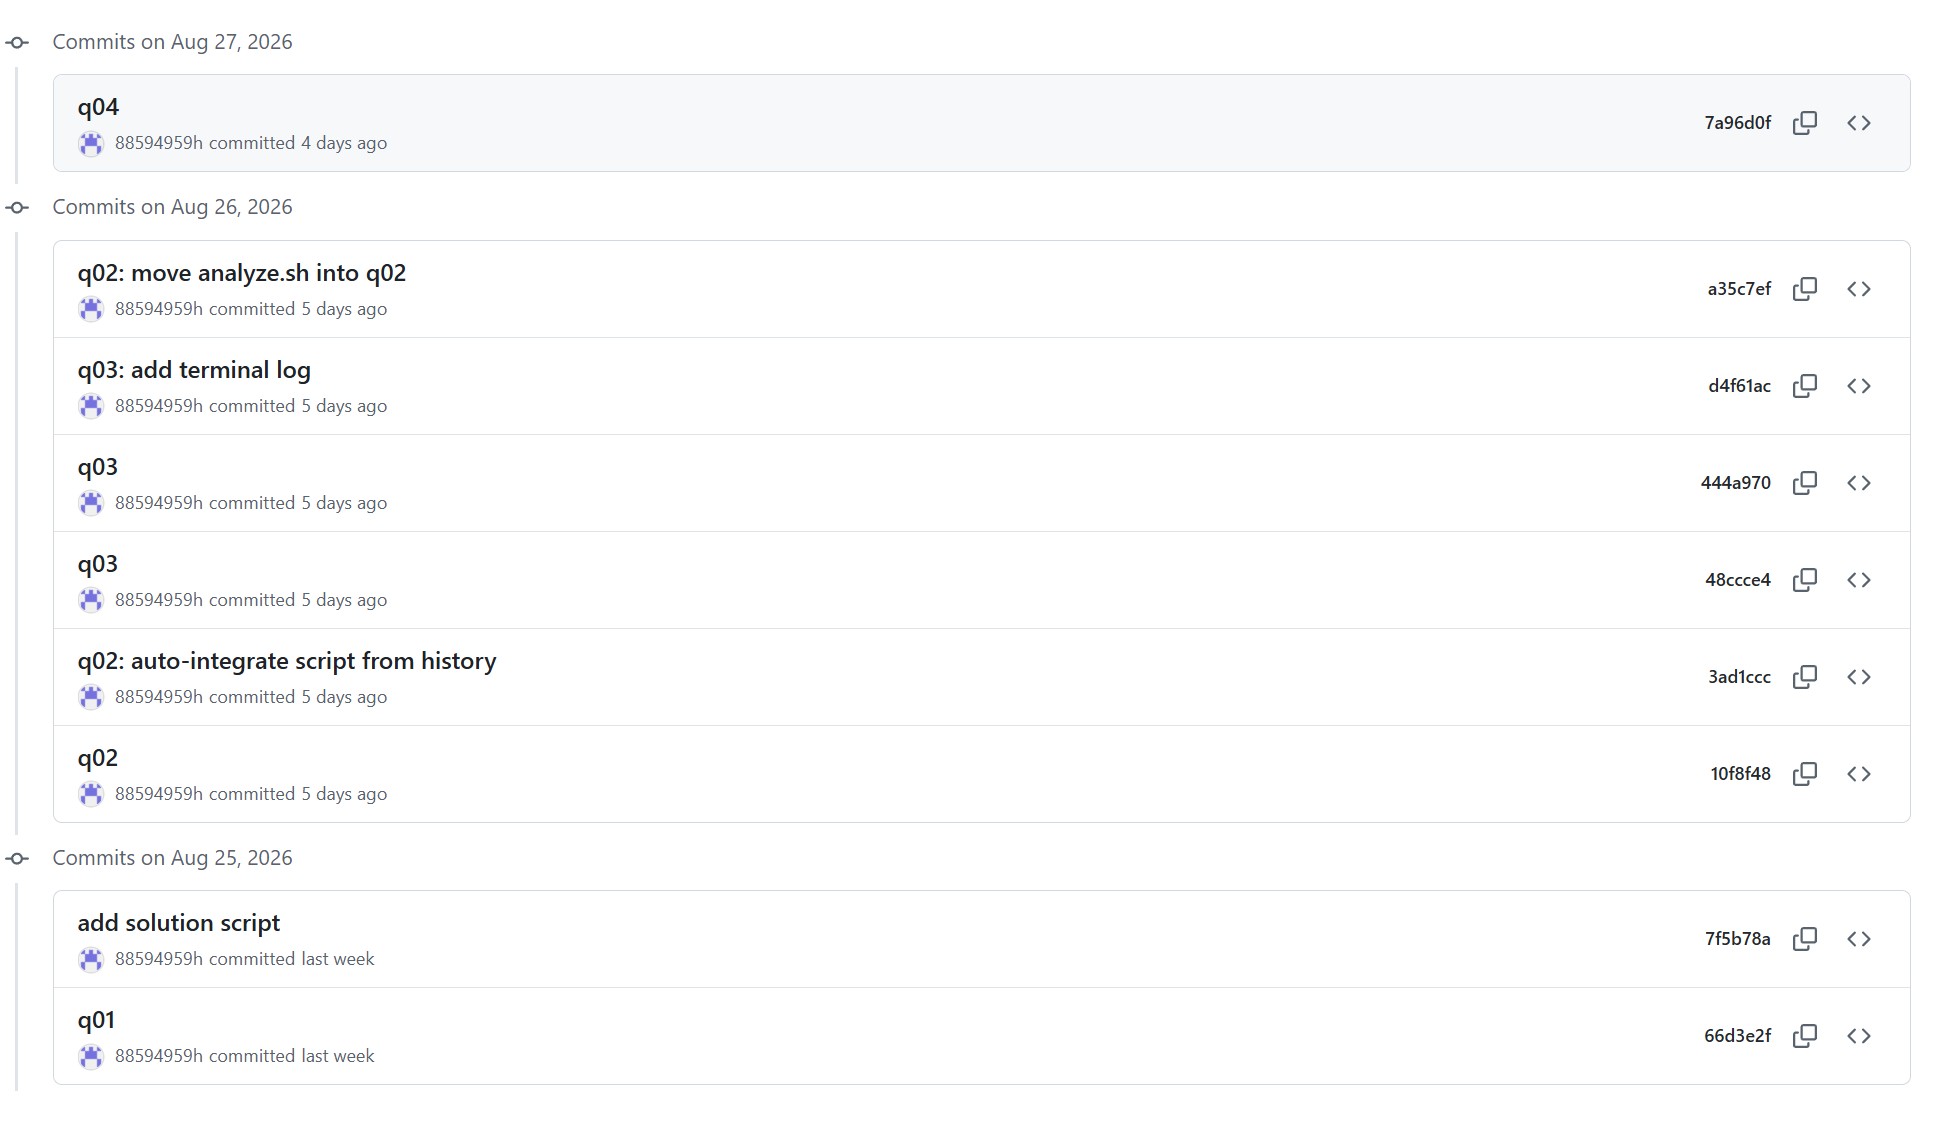
\includegraphics[width=0.9\textwidth]{commit_log.png}
    \captionsetup{labelfont={color=themeBlue,bf}, textfont={color=darkText}}
    \caption{Git Commit 历史记录截图（git log --oneline）}
    \label{fig:commit_log}
\end{figure}

% ==================== 课上实验部分 ====================
\newpage
\section{课上实验 (第 1 周)}

% ---------- 实验一 ----------
\subsection{实验一：含空格文件名的批量整理}

\subsubsection{题目要求}
\begin{enumerate}[leftmargin=2em]
    \item 创建 \texttt{input/docs} 和 \texttt{input/tmp}；创建含空格文件名的文件及隐藏文件。
    \item 显示 \texttt{q01} 的绝对路径，以长格式列出 \texttt{input} 下全部项目（含隐藏文件）。
    \item 将 \texttt{input} 下所有 \texttt{.txt} 文件复制到 \texttt{work/<学号>/}，保留相对目录结构并正确处理空格。
    \item 设置目录权限 750、文件权限 640；生成 \texttt{inventory.txt}。
\end{enumerate}

\subsubsection{核心指令与实现}
\begin{lstlisting}[caption={实验一关键 Shell 指令}]
# 1. 创建目录结构
mkdir -p input/docs input/tmp work/24170001032

# 2. 创建文件 (注意空格转义)
echo -e "alpha\nbeta" > "input/docs/notes one.txt"
echo "hidden" > input/docs/.secret.txt
touch input/tmp/empty.txt

# 3. 显示路径与列表
pwd
ls -la input/

# 4. 复制文件 (处理空格的关键: find + cp --parents 或 引号)
# 方法: 进入 input 目录操作以保持相对路径
(cd input && find . -name "*.txt" -exec cp --parents {} ../work/24170001032/ \;)

# 5. 设置权限
find work/24170001032 -type d -exec chmod 750 {} +
find work/24170001032 -type f -exec chmod 640 {} +

# 6. 生成 inventory.txt
(cd work/24170001032 && find . -type f -printf "%P %s\n" | sort > ../../inventory.txt)
\end{lstlisting}

\subsubsection{实验分析与难点}
\begin{infobox}[实现思路]
利用 \texttt{find} 命令配合 \texttt{-exec} 或管道来处理包含空格的文件名，避免直接使用通配符 \texttt{*} 导致的单词拆分问题。\texttt{cp --parents} 选项用于保留源文件的相对目录结构。
\end{infobox}

\begin{keybox}[实现重点]
\begin{itemize}
    \item \textbf{空格处理}：在 Shell 中，文件名含空格必须用双引号包裹，或使用 \texttt{find -print0 | xargs -0} 范式。
    \item \textbf{权限理解}：目录 750 (rwxr-x---) 允许所有者读写执行，组用户读执行；文件 640 (rw-r-----) 允许所有者读写，组用户只读。
\end{itemize}
\end{keybox}

\subsubsection{运行结果}

\begin{figure}[H]
    \centering
    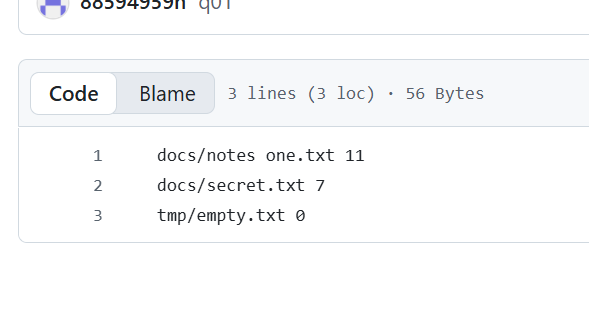
\includegraphics[width=0.9\textwidth]{屏幕截图 2026-09-01 225601.png}
    \captionsetup{labelfont={color=themeBlue,bf}, textfont={color=darkText}}
    \caption{实验一：inventory.txt 内容截图}
\end{figure}
% ---------- 实验二 ----------
\newpage
\subsection{实验二：随机访问日志统计}

\subsubsection{题目要求}
在 \texttt{q02} 中创建 \texttt{access.csv}，并使用下方给定数据完成日志统计。
\textbf{给定内容（access.csv）：}
\begin{lstlisting}
timestamp,user,path,status,latency_ms
09:00:01,alice,/api/users,200,120
09:00:02,bob,/api/orders,500,310
09:00:03,alice,/api/users,503,180
09:00:04,carol,/login,500,90
09:00:05,bob,/api/orders,502,260
09:00:06,dave,/health,200,20
09:00:07,alice,/api/orders,500,420
09:00:08,carol,/api/users,500,150
\end{lstlisting}

\begin{enumerate}[leftmargin=2em]
    \item 编写 \texttt{analyze.sh}，接收一个 CSV 文件路径；文件不存在时将错误写入 stderr 并返回非零退出码。
    \item 使用 Shell 管道以及 \texttt{awk}、\texttt{sort}、\texttt{head} 等工具，输出 HTTP 5xx 数量最多的前 2 个 path；按次数降序，次数相同时按 path 字典序。
    \item 输出全部数据行的平均 \texttt{latency\_ms}，保留两位小数；表头不得计入。
    \item 分别对 \texttt{access.csv} 和一个不存在的文件运行脚本；不得使用 Python、电子表格或手工统计。
\end{enumerate}

\subsubsection{脚本实现 (analyze.sh)}
\begin{lstlisting}[caption={analyze.sh 脚本内容}]
#!/bin/bash
FILE=$1

# 检查文件是否存在
if [ ! -f "$FILE" ]; then
    echo "Error: File '$FILE' not found." >&2
    exit 1
fi

echo "=== Top 2 Paths with 5xx Errors ==="
# 跳过表头，筛选 5xx 状态码 (第4列)，提取 path (第3列)，排序统计
tail -n +2 "$FILE" | awk -F',' '$4 ~ /^5/ {print $3}' | sort | uniq -c | sort -rn -k1,1 -k2,2 | head -n 2

echo ""
echo "=== Average Latency ==="
# 计算平均 latency (第5列)，保留两位小数
tail -n +2 "$FILE" | awk -F',' '{sum+=$5; count++} END {if(count>0) printf "%.2f\n", sum/count; else print "0.00"}'
\end{lstlisting}

\subsubsection{运行结果}
\begin{lstlisting}[caption={正常文件运行结果}]
$ ./analyze.sh access.csv
=== Top 2 Paths with 5xx Errors ===
      2 /api/orders
      1 /api/users

=== Average Latency ===
193.75
\end{lstlisting}

\begin{lstlisting}[caption={异常文件运行结果}]
$ ./analyze.sh nonexistent.csv
Error: File 'nonexistent.csv' not found.
$ echo $?
1
\end{lstlisting}

% ---------- 实验三 ----------
\newpage
\subsection{实验三：制造、解决并解释一次合并冲突}

\subsubsection{题目要求}
在 \texttt{q03} 中从零创建一个 Git 仓库，并主动制造、解决一次合并冲突。
\begin{enumerate}[leftmargin=2em]
    \item 初始化仓库，在 \texttt{main} 创建 \texttt{config.txt}，内容为 \texttt{mode=normal}，并完成初始提交。
    \item 创建 \texttt{feature-a}，把内容改为 \texttt{mode=safe} 并提交；从初始 \texttt{main} 创建 \texttt{feature-b}，把内容改为 \texttt{mode=fast} 并提交。
    \item 回到 \texttt{main}，先合并 \texttt{feature-a}，再合并 \texttt{feature-b}；解决冲突时保留 \texttt{mode=safe}，并另加一行 \texttt{note=reviewed}。
    \item 确认工作区干净，运行 \texttt{git log --all --graph --decorate --oneline} 查看历史。
\end{enumerate}

\subsubsection{Git 操作流程}
\begin{lstlisting}[caption={Git 操作指令序列}]
# 1. 初始化与初始提交
git init -b main
echo "mode=normal" > config.txt
git add config.txt
git commit -m "Initial commit with mode=normal"

# 2. Feature A 分支
git checkout -b feature-a
echo "mode=safe" > config.txt
git add config.txt
git commit -m "Change mode to safe in feature-a"

# 3. Feature B 分支 (从 main 分出)
git checkout main
git checkout -b feature-b
echo "mode=fast" > config.txt
git add config.txt
git commit -m "Change mode to fast in feature-b"

# 4. 合并与冲突解决
git checkout main
git merge feature-a  # Fast-forward 成功
git merge feature-b  # 产生 CONFLICT

# 5. 手动解决冲突
echo "mode=safe" > config.txt
echo "note=reviewed" >> config.txt
git add config.txt
git commit -m "Merge feature-b: resolve conflict, keep safe mode"

# 6. 查看历史
git log --all --graph --decorate --oneline
\end{lstlisting}

\subsubsection{冲突解决分析}
\begin{infobox}[原理说明]
当两个分支修改了同一文件的同一行时，Git 无法自动合并，会标记冲突。此时文件中会出现 \texttt{<<<<<<<}, \texttt{=======}, \texttt{>>>>>>>} 标记。我们需要手动编辑文件保留 desired content，然后 \texttt{git add} 标记为已解决，最后 \texttt{git commit} 完成合并。
\end{infobox}

\subsubsection{运行结果}
\begin{lstlisting}[caption={Git Log 图形化输出}]
* a616d51 (HEAD -> main) Merge feature-b: resolve conflict...

|\
| * 3f9b85f (feature-b) Change mode to fast in feature-b
* | 71f7c45 (feature-a) Change mode to safe in feature-a

|/
* 1d8c934 Initial commit with mode=normal
\end{lstlisting}

% ---------- 实验四 ----------
\newpage
\subsection{实验四：修复并构建一页技术说明 (LaTeX)}

\subsubsection{题目要求}
补全 LaTeX 模板，加入公式、表格及交叉引用，使用 \texttt{latexmk} 生成 PDF。

\subsubsection{实现代码片段}
\begin{lstlisting}[caption={report.tex 关键片段}]
\section{Result}
爱因斯坦质能方程如公式 \eqref{eq:einstein} 所示：
\begin{equation}
    E = mc^2
    \label{eq:einstein}
\end{equation}

实验数据汇总见表 \ref{tab:data}。
\begin{table}[H]
    \centering
    \caption{实验数据记录}
    \label{tab:data}
    \begin{tabular}{cc}
        \toprule
        \textbf{变量} & \textbf{值} \\
        \midrule
        Mass & 1.0 kg \\
        Energy & 9.0e16 J \\
        \bottomrule
    \end{tabular}
\end{table}
\end{lstlisting}

\subsubsection{编译指令}
\begin{lstlisting}[caption={编译命令}]
latexmk -pdf -halt-on-error report.tex
\end{lstlisting}

\subsubsection{运行结果}

\begin{figure}[H]
    \centering
    
\includegraphics[width=0.9\textwidth]{屏幕截图 2026-09-01 221413.png}
    \captionsetup{labelfont={color=themeBlue,bf}, textfont={color=darkText}}
    \caption{实验四：生成的 PDF 页面截图}
\end{figure}

% ==================== 课后思考题 ====================
\newpage
\section{课后思考题}

% ---------- 题 1 ----------
\subsection{思考题 1：标准流重定向}
\textbf{题目}：运行 \texttt{ls /nonexistent /tmp}，把 stdout 和 stderr 分别重定向到两个文件。如何将两者都重定向到同一个文件？

\textbf{解答}：
\begin{lstlisting}
# 分别重定向
ls /nonexistent /tmp > out.txt 2> err.txt

# 合并重定向 (2>&1 表示将 stderr 指向 stdout 当前指向的地方)
ls /nonexistent /tmp > all.txt 2>&1
\end{lstlisting}

\begin{figure}[H]
    \centering
    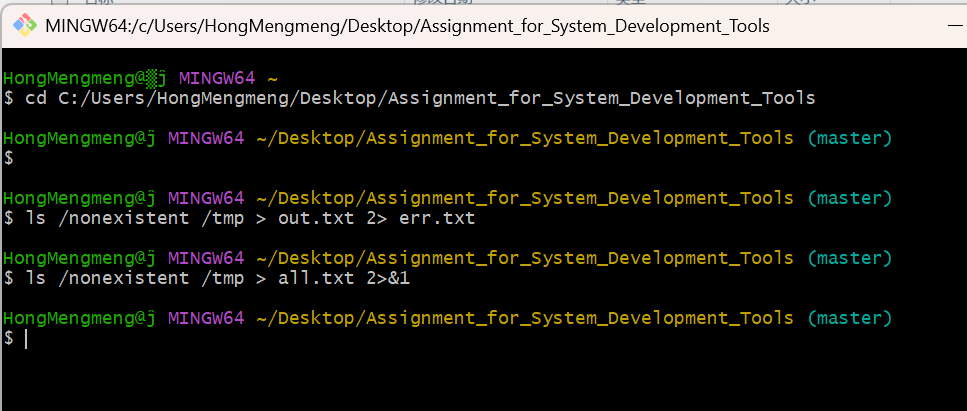
\includegraphics[width=0.9\textwidth]{屏幕截图 2026-09-01 222946.png}
    \captionsetup{labelfont={color=themeBlue,bf}, textfont={color=darkText}}
    \caption{两种情况示例}
\end{figure}
\begin{figure}[H]
    \centering
    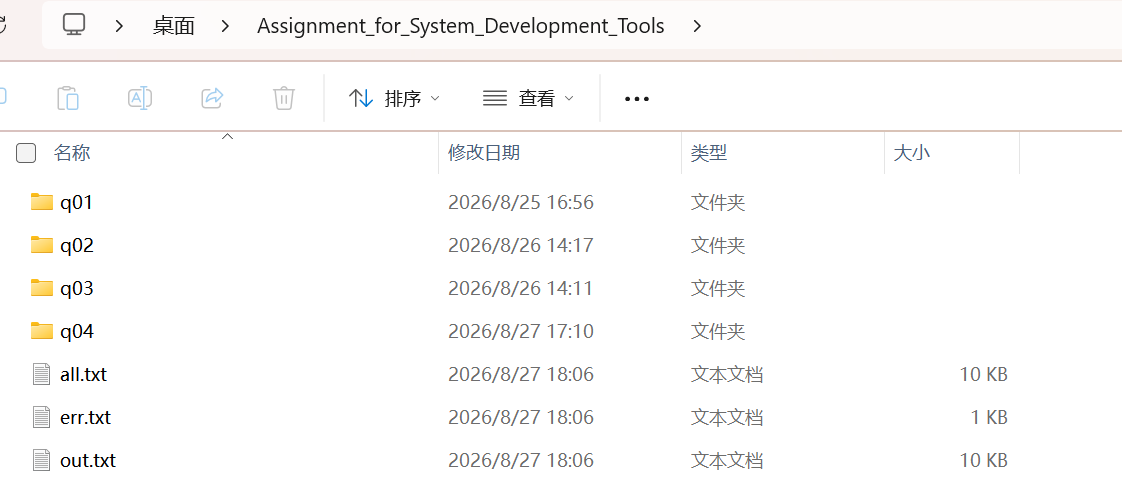
\includegraphics[width=0.9\textwidth]{屏幕截图 2026-08-27 180735.png}
    \captionsetup{labelfont={color=themeBlue,bf}, textfont={color=darkText}}
    \caption{变化情况1}
\end{figure}
\begin{figure}[H]
    \centering
    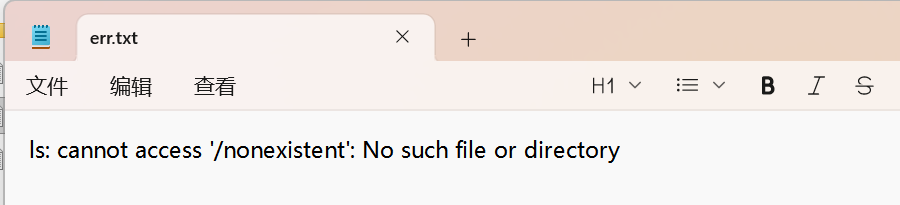
\includegraphics[width=0.9\textwidth]{屏幕截图 2026-08-27 180846.png}
    \captionsetup{labelfont={color=themeBlue,bf}, textfont={color=darkText}}
    \caption{变化情况2}
\end{figure}

% ---------- 题 2 ----------
\subsection{思考题 2：条件执行与目录创建}
\textbf{题目}：写一个一行命令：仅当 \texttt{/tmp/mydir} 不存在时才创建它。

\textbf{解答}：
利用 \texttt{||} (OR) 操作符，前一条命令失败（即目录不存在，测试返回非0）时执行后一条。
\begin{lstlisting}
[ -d /tmp/mydir ] || mkdir /tmp/mydir
\end{lstlisting}
或者使用更简洁的 \texttt{mkdir -p} (虽不完全是题目要求的逻辑，但效果类似且幂等)。

\begin{figure}[H]
    \centering
    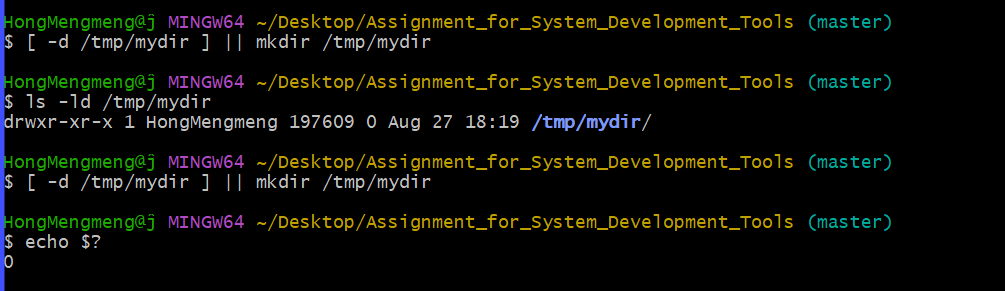
\includegraphics[width=0.9\textwidth]{屏幕截图 2026-08-27 182008.png}
    \captionsetup{labelfont={color=themeBlue,bf}, textfont={color=darkText}}
    \caption{第一次及第二次运行}
\end{figure}
\begin{figure}[H]
    \centering
    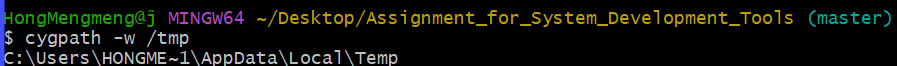
\includegraphics[width=0.9\textwidth]{屏幕截图 2026-08-27 182514.png}
    \captionsetup{labelfont={color=themeBlue,bf}, textfont={color=darkText}}
    \caption{绝对路径}
\end{figure}
% ---------- 题 3 ----------
\subsection{思考题 3：cd 为什么必须是内建命令}
\textbf{题目}：为什么 \texttt{cd} 必须是 Shell 内建命令，而不能是独立程序？

\textbf{解答}：
\begin{keybox}[核心原因]
\textbf{子进程不能改变父进程的工作目录。}
Shell 执行外部命令时会 \texttt{fork} 一个子进程。子进程结束后，其对环境（包括当前工作目录 CWD）的任何修改都会随之消失，无法回传给父进程（Shell）。如果 \texttt{cd} 是外部程序，它只能改变自己子进程的目录，Shell 本身的目录不会变，命令也就失去了意义。因此，\texttt{cd} 必须由 Shell 自己在内部执行。
\end{keybox}

\begin{figure}[H]
    \centering
    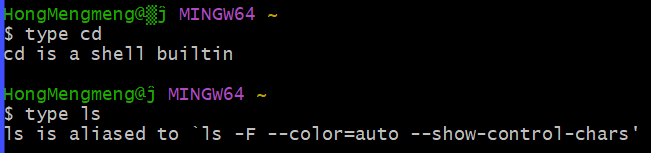
\includegraphics[width=0.9\textwidth]{屏幕截图 2026-08-27 183022.png}
    \captionsetup{labelfont={color=themeBlue,bf}, textfont={color=darkText}}
    \caption{运行示例}
\end{figure}

% ---------- 题 4 ----------
\subsection{思考题 4：文件存在性检查脚本}
\textbf{题目}：写一个脚本，接收文件名参数，检查是否存在并输出提示。

\textbf{解答}：
\begin{lstlisting}
#!/bin/bash
if [ -f "$1" ]; then
    echo "File '$1' exists."
else
    echo "File '$1' does not exist."
fi
\end{lstlisting}

\begin{figure}[H]
    \centering
    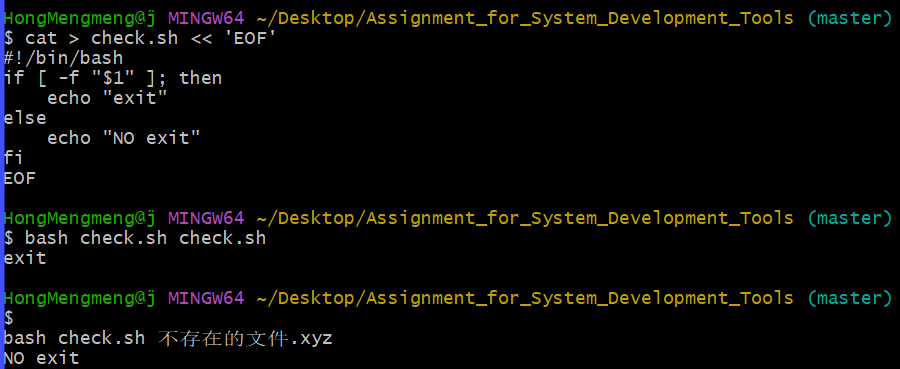
\includegraphics[width=0.9\textwidth]{屏幕截图 2026-08-27 184445.png}
    \captionsetup{labelfont={color=themeBlue,bf}, textfont={color=darkText}}
    \caption{运行示例}
\end{figure}

% ---------- 题 5 ----------
\subsection{思考题 5：set -x 的作用}
\textbf{题目}：在脚本的 \texttt{set} 选项里加入 \texttt{-x} 会发生什么？

\textbf{解答}：
\texttt{set -x} 开启 \textbf{执行追踪 (Execution Tracing)} 模式。Shell 在执行每条命令前，会将其（展开变量后）打印到 stderr，并以 \texttt{+} 开头。这是调试脚本最有效的手段，可以清晰看到变量的真实值和命令的执行流程。

\begin{figure}[H]
    \centering
    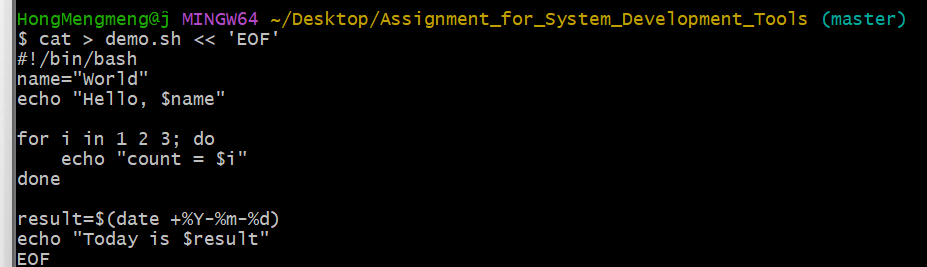
\includegraphics[width=0.9\textwidth]{屏幕截图 2026-08-28 083838.png}
    \captionsetup{labelfont={color=themeBlue,bf}, textfont={color=darkText}}
    \caption{创建一个简单的脚本文件}
\end{figure}
\begin{figure}[H]
    \centering
    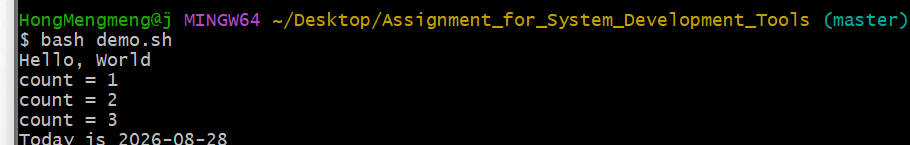
\includegraphics[width=0.9\textwidth]{屏幕截图 2026-08-28 083911.png}
    \captionsetup{labelfont={color=themeBlue,bf}, textfont={color=darkText}}
    \caption{普通输出}
\end{figure}
\begin{figure}[H]
    \centering
    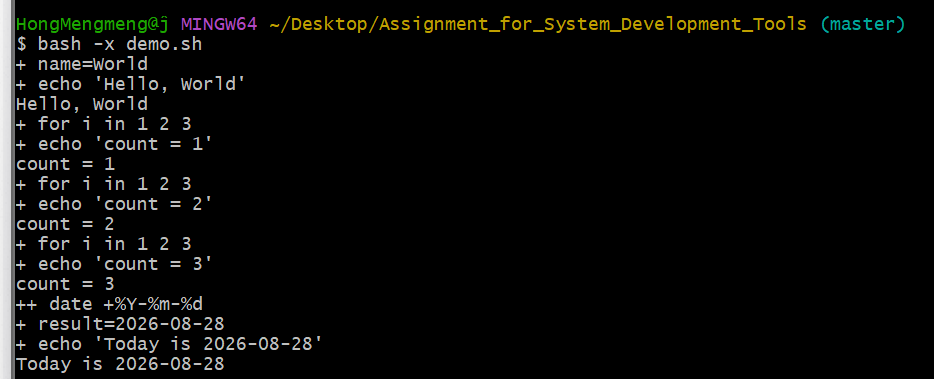
\includegraphics[width=0.9\textwidth]{屏幕截图 2026-08-28 084004.png}
    \captionsetup{labelfont={color=themeBlue,bf}, textfont={color=darkText}}
    \caption{加上-x输出}
\end{figure}
% ---------- 题 6 ----------
\subsection{思考题 6：带日期的文件备份}
\textbf{题目}：写一条命令，把文件复制为带当天日期的备份文件名。

\textbf{解答}：
利用命令替换 \texttt{\$(...)} 获取日期。
\begin{lstlisting}
cp notes.txt notes_$(date +%Y-%m-%d).txt
\end{lstlisting}

\begin{figure}[H]
    \centering
    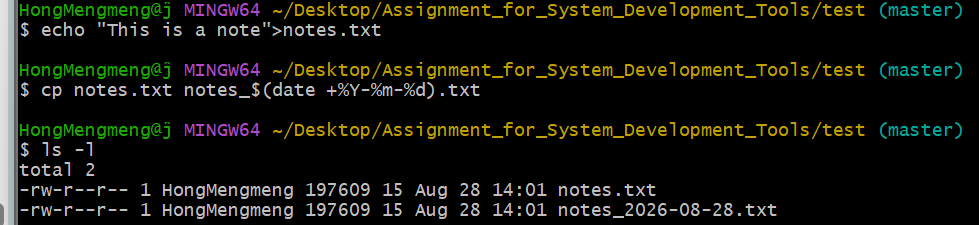
\includegraphics[width=0.9\textwidth]{屏幕截图 2026-08-28 140148.png}
    \captionsetup{labelfont={color=themeBlue,bf}, textfont={color=darkText}}
    \caption{运行示例}
\end{figure}
% ---------- 题 7 ----------
\subsection{思考题 7：统计常见文件扩展名}
\textbf{题目}：使用管道找出 home 目录中最常见的 5 种文件扩展名。

\textbf{解答}：
\begin{lstlisting}
find ~ -type f | grep -oE '\.[a-zA-Z0-9]+$' | sort | uniq -c | sort -rn | head -5
\end{lstlisting}
\textbf{解析}：\texttt{find} 找文件 $\to$ \texttt{grep} 提取扩展名 $\to$ \texttt{sort} 排序 $\to$ \texttt{uniq -c} 计数 $\to$ \texttt{sort -rn} 降序 $\to$ \texttt{head} 取前5。

\begin{figure}[H]
    \centering
    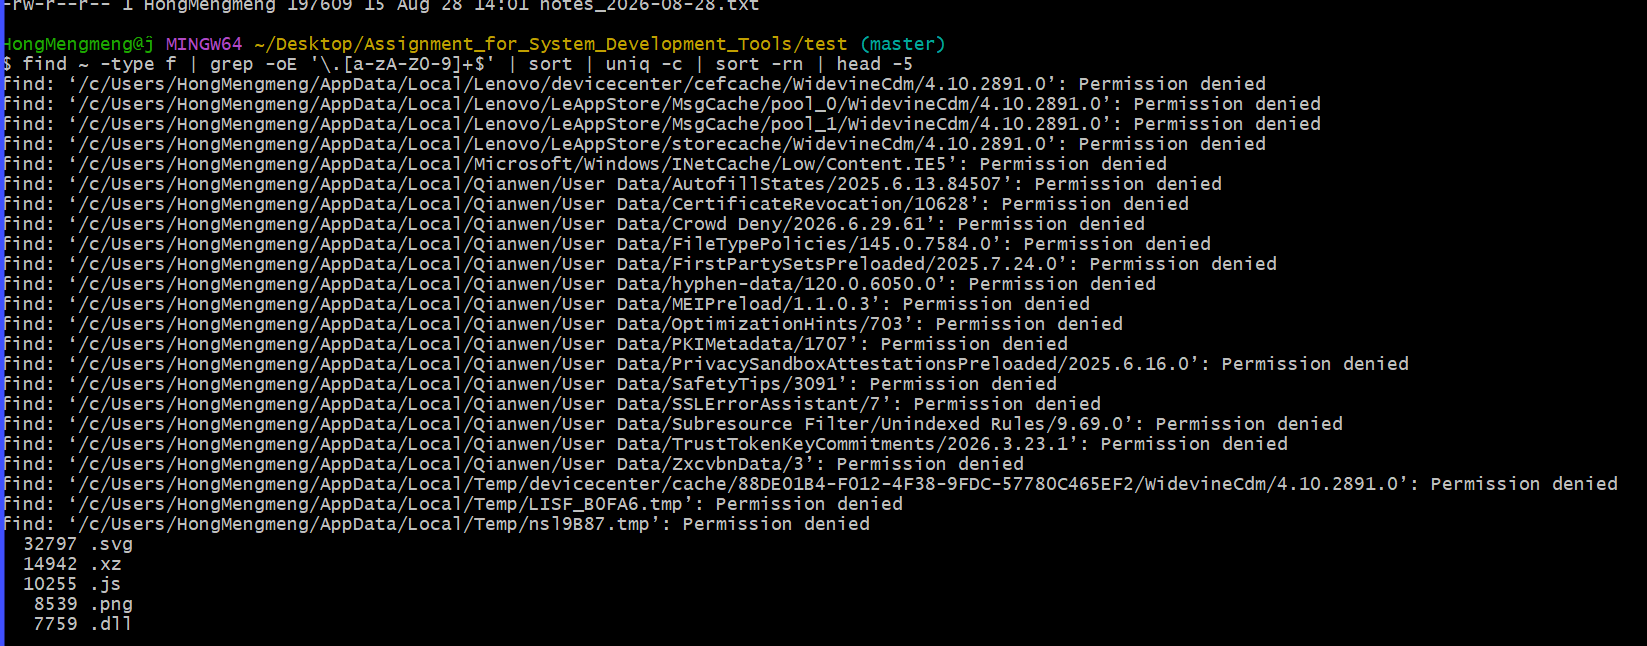
\includegraphics[width=0.9\textwidth]{屏幕截图 2026-08-28 155118.png}
    \captionsetup{labelfont={color=themeBlue,bf}, textfont={color=darkText}}
    \caption{运行示例}
\end{figure}
% ---------- 题 8 ----------
\subsection{思考题 8：xargs 与空格处理}
\textbf{题目}：结合 \texttt{find} 和 \texttt{xargs} 统计 .sh 文件行数，正确处理空格。

\textbf{解答}：
使用 \texttt{-print0} 和 \texttt{-0} 配对，以 NULL 字符分隔，彻底避免空格/换行符干扰。
\begin{lstlisting}
find ~ -type f -name '*.sh' -print0 | xargs -0 wc -l
\end{lstlisting}

\begin{figure}[H]
    \centering
    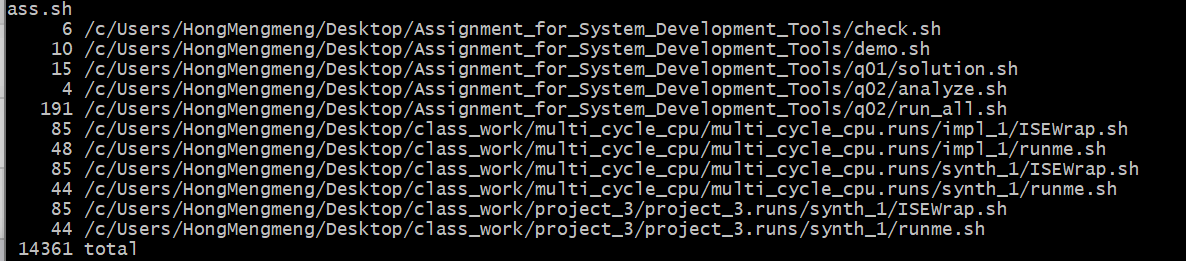
\includegraphics[width=0.9\textwidth]{屏幕截图 2026-08-28 160321.png}
    \captionsetup{labelfont={color=themeBlue,bf}, textfont={color=darkText}}
    \caption{统计结果}
\end{figure}
% ---------- 题 9 ----------
\subsection{思考题 9：Shell 引用机制}
\textbf{题目}：单引号、双引号和 ANSI-C 引号的区别？输出含 \texttt{\$}, \texttt{!}, 换行符的字符串。

\textbf{解答}：
\begin{itemize}
    \item \textbf{单引号 \texttt{'...'}}：强引用，内容完全原样输出，不解析任何变量或转义。
    \item \textbf{双引号 \texttt{"..."}}：弱引用，解析变量 \texttt{\$var} 和命令替换 \texttt{\$(cmd)}，但保留空格。
    \item \textbf{ANSI-C \texttt{\$'...'}}：支持 C 风格转义，如 \texttt{\textbackslash n} (换行), \texttt{\textbackslash t} (制表符)。
\end{itemize}

\textbf{命令}：
\begin{lstlisting}
echo $'Price is \$100!\nNew Line here.'
\end{lstlisting}
\begin{figure}[H]
    \centering
    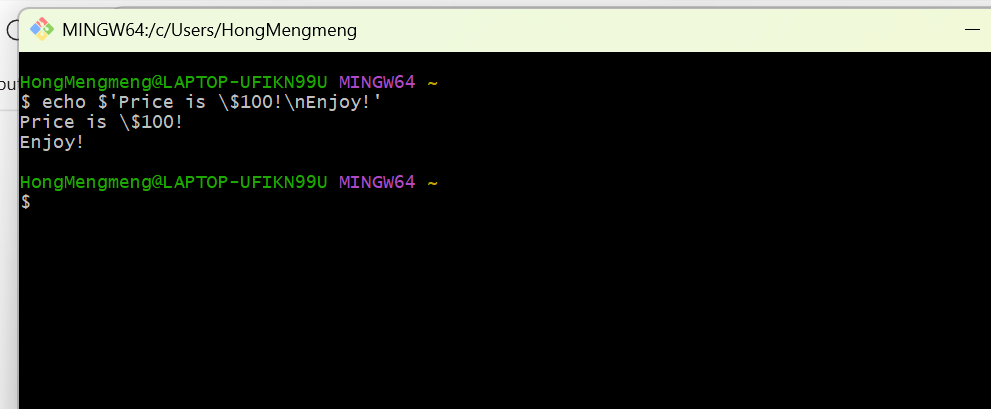
\includegraphics[width=0.9\textwidth]{屏幕截图 2026-08-25 152029.png}
    \captionsetup{labelfont={color=themeBlue,bf}, textfont={color=darkText}}
    \caption{运行示例}
\end{figure}
% ---------- 题 10 ----------
\subsection{思考题 10：Glob 模式匹配}
\textbf{题目}：什么是 glob？测试 \texttt{ls *.txt} 等模式。

\textbf{解答}：
Glob 是 Shell 内置的文件名通配符匹配机制，由 Shell 在命令执行前展开为文件列表。
\begin{itemize}
    \item \texttt{*}：匹配任意长度字符串（不含 /）。
    \item \texttt{?}：匹配单个字符。
    \item \texttt{[abc]}：匹配括号内任一字符。
    \item \texttt{\{a,b\}}：花括号展开（Brace Expansion），生成多个参数。
\end{itemize}
注意：Glob 不是正则表达式，它只用于匹配文件名。

\begin{figure}[H]
    \centering
    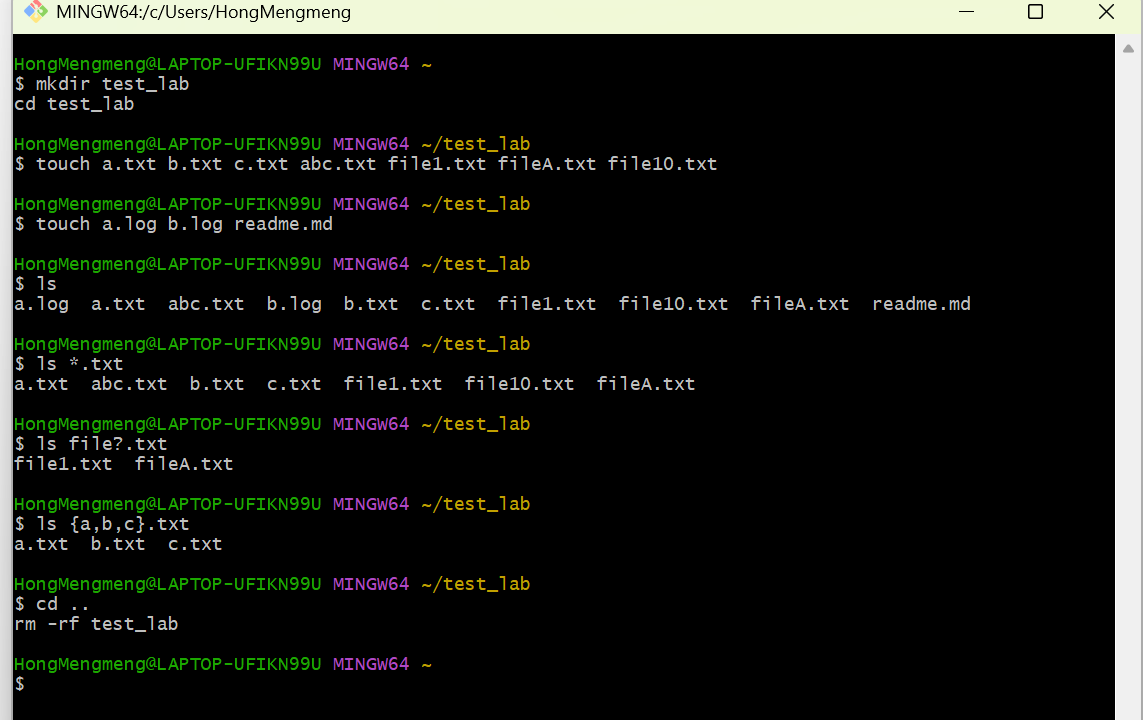
\includegraphics[width=0.9\textwidth]{屏幕截图 2026-08-25 150001.png}
    \captionsetup{labelfont={color=themeBlue,bf}, textfont={color=darkText}}
    \caption{运行示例}
\end{figure}

% ---------- 题 11 ----------
\subsection{思考题 11：ls -l 输出格式解析}
\textbf{题目}：\texttt{ls} 的 \texttt{-l} 选项（flag）作用是什么？运行 \texttt{ls -l /} 并观察输出。每一行最前面的 10 个字符分别代表什么？

\textbf{解答}：
\begin{keybox}[ls -l 的作用]
\texttt{ls -l} 以\textbf{长格式（long listing）}显示文件或目录的详细信息，包括：文件类型与权限、硬链接数、所有者、所属组、文件大小（字节）、最后修改时间、文件名（或目录名）。
\end{keybox}

\begin{figure}[H]
    \centering
    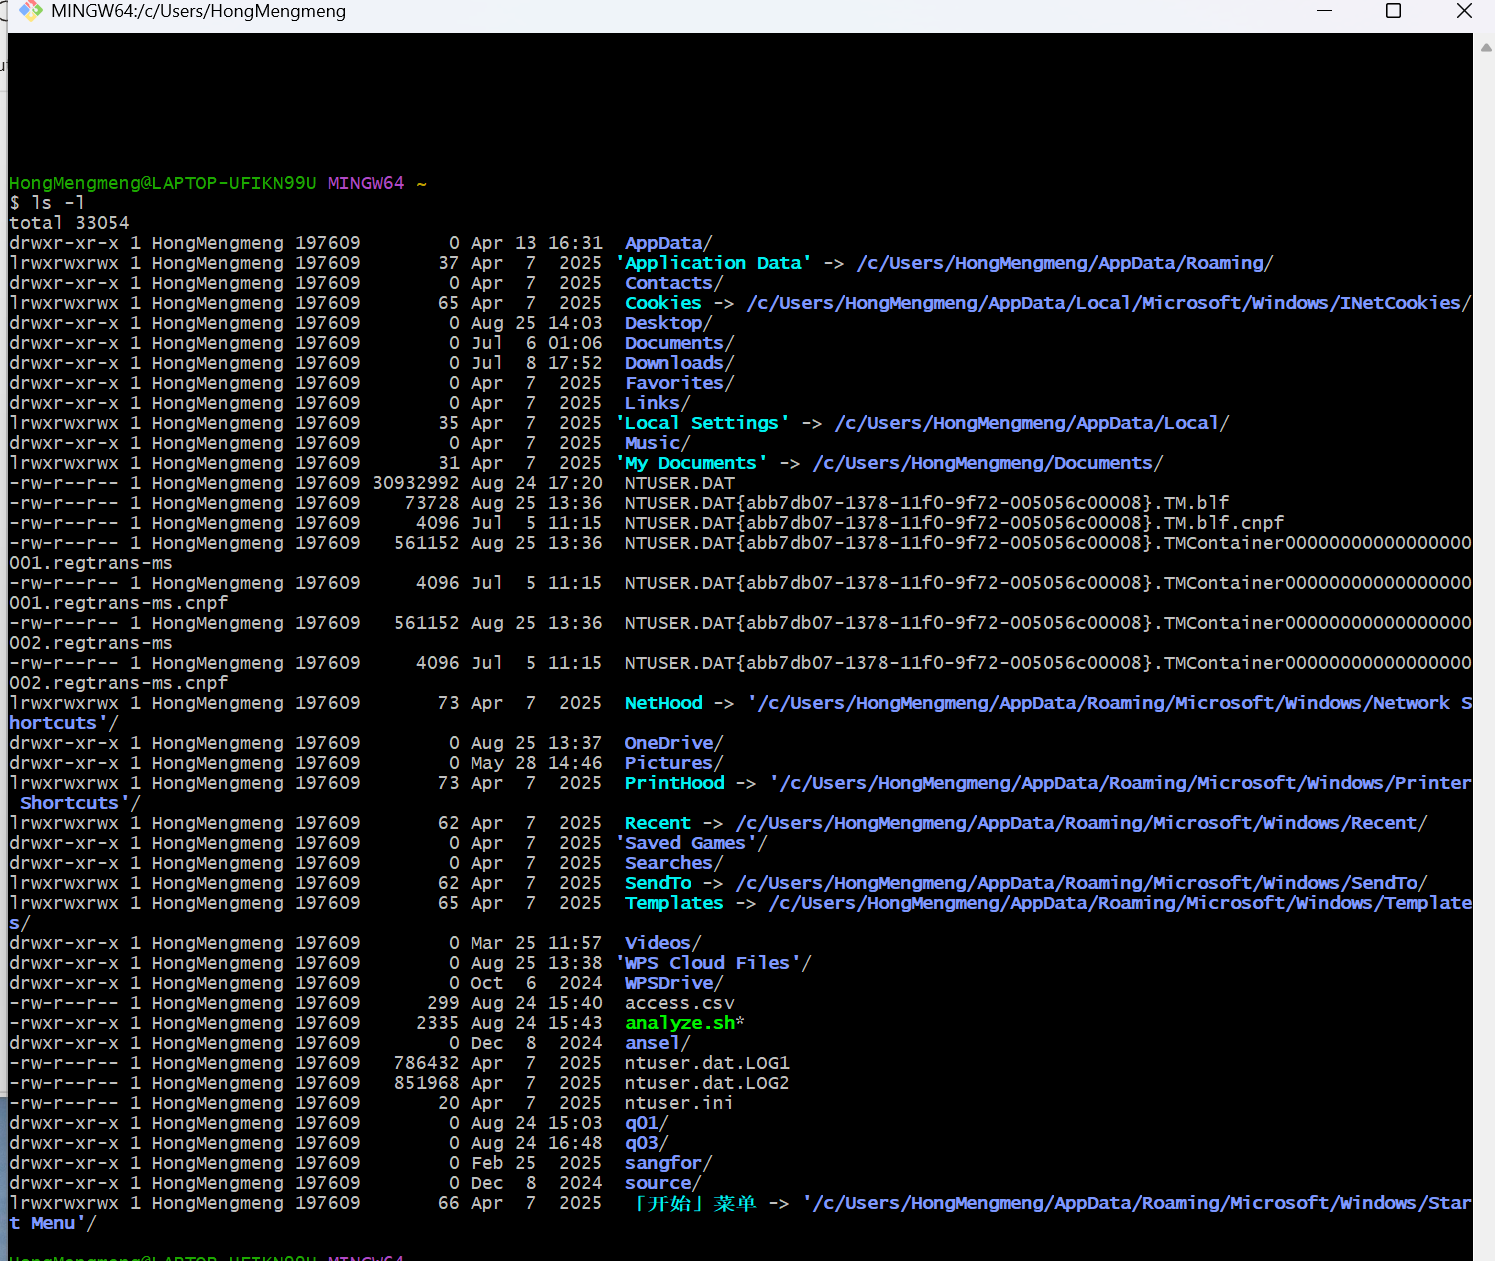
\includegraphics[width=0.9\textwidth]{屏幕截图 2026-08-25 143625.png}
    \captionsetup{labelfont={color=themeBlue,bf}, textfont={color=darkText}}
    \caption{输出示例}
\end{figure}
每行最前面 \textbf{10 个字符}的含义如下：
\medskip
\noindent\textbf{第 1 位：文件类型}
\begin{center}
\small
\begin{tabular}{cl}
    \toprule
    \textbf{字符} & \textbf{含义} \\
    \midrule
    \texttt{d} & 目录（directory） \\
    \texttt{-} & 普通文件（regular file） \\
    \texttt{l} & 符号链接（symbolic link） \\
    \texttt{c} & 字符设备（character device） \\
    \texttt{b} & 块设备（block device） \\
    \texttt{p} & 命名管道（named pipe / FIFO） \\
    \texttt{s} & 套接字（socket） \\
    \bottomrule
\end{tabular}
\end{center}
\medskip
\noindent\textbf{第 2--10 位：权限位（3 组 × 3 位）}
\begin{itemize}[leftmargin=2em, itemsep=3pt]
    \item \textbf{第 2--4 位}：所有者（user）权限
    \item \textbf{第 5--7 位}：所属组（group）权限
    \item \textbf{第 8--10 位}：其他人（others）权限
\end{itemize}
每组三位依次为 \texttt{r}（读）、\texttt{w}（写）、\texttt{x}（执行）；对应位置为 \texttt{-} 表示无该权限。例如 \texttt{-rw-r--r--} 表示：普通文件，所有者可读写，组用户和其他人仅可读。
% ==================== 实验总结 ====================
\newpage
\section{实验总结与感悟}

\subsection{遇到的问题与解决方法}
\begin{enumerate}
    \item \textbf{文件名空格问题}：在实验一中，直接使用 \texttt{cp input/docs/*.txt} 会导致含空格的文件名被截断。通过改用 \texttt{find ... -exec} 或给变量加双引号 \texttt{"\$file"} 解决。
    \item \textbf{Git 冲突标记}：初次遇到冲突时不知所措，通过查阅文档理解了 \texttt{<<<<<<<} 标记的含义，手动编辑文件后记得 \texttt{git add} 才能标记为已解决。
    \item \textbf{LaTeX 字体报错}：最初手动指定 \texttt{SimSun} 导致编译失败，改为依赖 \texttt{ctex} 自动检测系统字体后解决。
\end{enumerate}

\subsection{心得体会}
通过本次实验，我深刻体会到了命令行工具的强大之处。特别是管道 \texttt{|} 的设计哲学——“每个程序只做一件事，并做好”，通过组合小工具完成复杂任务（如题7的统计），比编写庞大的单体程序更高效。同时，Git 的分支与合并机制让我理解了版本控制在协作中的核心价值。LaTeX 虽然上手有门槛，但其对学术排版的严谨性令人印象深刻。



\end{document}